%
\section{Data Base design}

Around the world there are a lot of different types of data bases [1]. However we used mySQL most popular – relational data base. Relational data bases are easily understand [2] and use. In general relational data bases - collection of relations and also it fit all our requirements.

\subsection{Why MySQL?}

Amount of different relational data bases are huge [3] and sometimes are difficult to choose. Our choice was MySQL data base, because it is:

\begin{itemize}
	\item Open source data base
	\item Ease to use
	\item Fast performance
	\item Reliable 
	\item Most popular open source DB in the world
	\item It is used by Yahoo!, Alcatel-Lucent, Google, Nokia, YouTube and others
\end{itemize}

\subsection{ER diagram}

Design of the data base mostly starts from modeling data base. One of the most popular approaches is conceptual modeling by using entity relational diagram (ER) [4]. Entity relational diagram shows collections of relations in modeling database. ER diagram allow easily understand concept of the data base. Another methodology to model data base can be used UML diagram. Most of the OOP programmers are familiar to UML and it make so popular. In our design we used ER diagram and later it were converted to UML [Appendix B].

\begin{figure}[h]
	\centering
		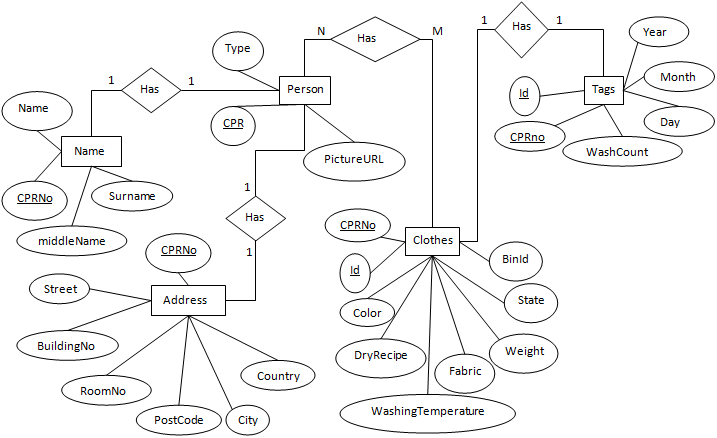
\includegraphics{erDiagramSmall}
	\caption{Laundry ER diagram}
	\label{fig:planning}
\end{figure}

\subsection{Implementation}

Make data base to work we need create tables and move them into data base. Data base tables were created by using query language like shown in the figure 5.1. All the code was written into text file and text file uploaded directly to data base by using created configurator tool.

\begin{figure}[h]
	\centering
		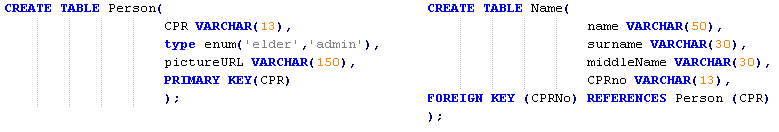
\includegraphics{personAndNamesTable}
	\caption{Person and Name tables}
	\label{fig:planning}
\end{figure}

Table person have three attributes: CPR, type and pictureURL and primary key for CPR. Primary key makes table to be unique, without a key table become weak entity type, note that always is good to have tables of strong entity types [4]. Foreign key makes table name also unique. In other words table name have one unique reference to table person and table person is unique. \\ Make easy for data base management were created data base configurator, which is able connect to data base and configure by query language or send files with configuration sentences. This manner let faster update and change without writing. 

\subsection{Future work}

Usage of all tables is not optimal and some attributes do not used at all so space usage can be decreased.
Speed increased